\section{Appendix for eksempler}
\subsection{Newton Euler dynamics and COM}
\begin{figure}[H]
    \centering
    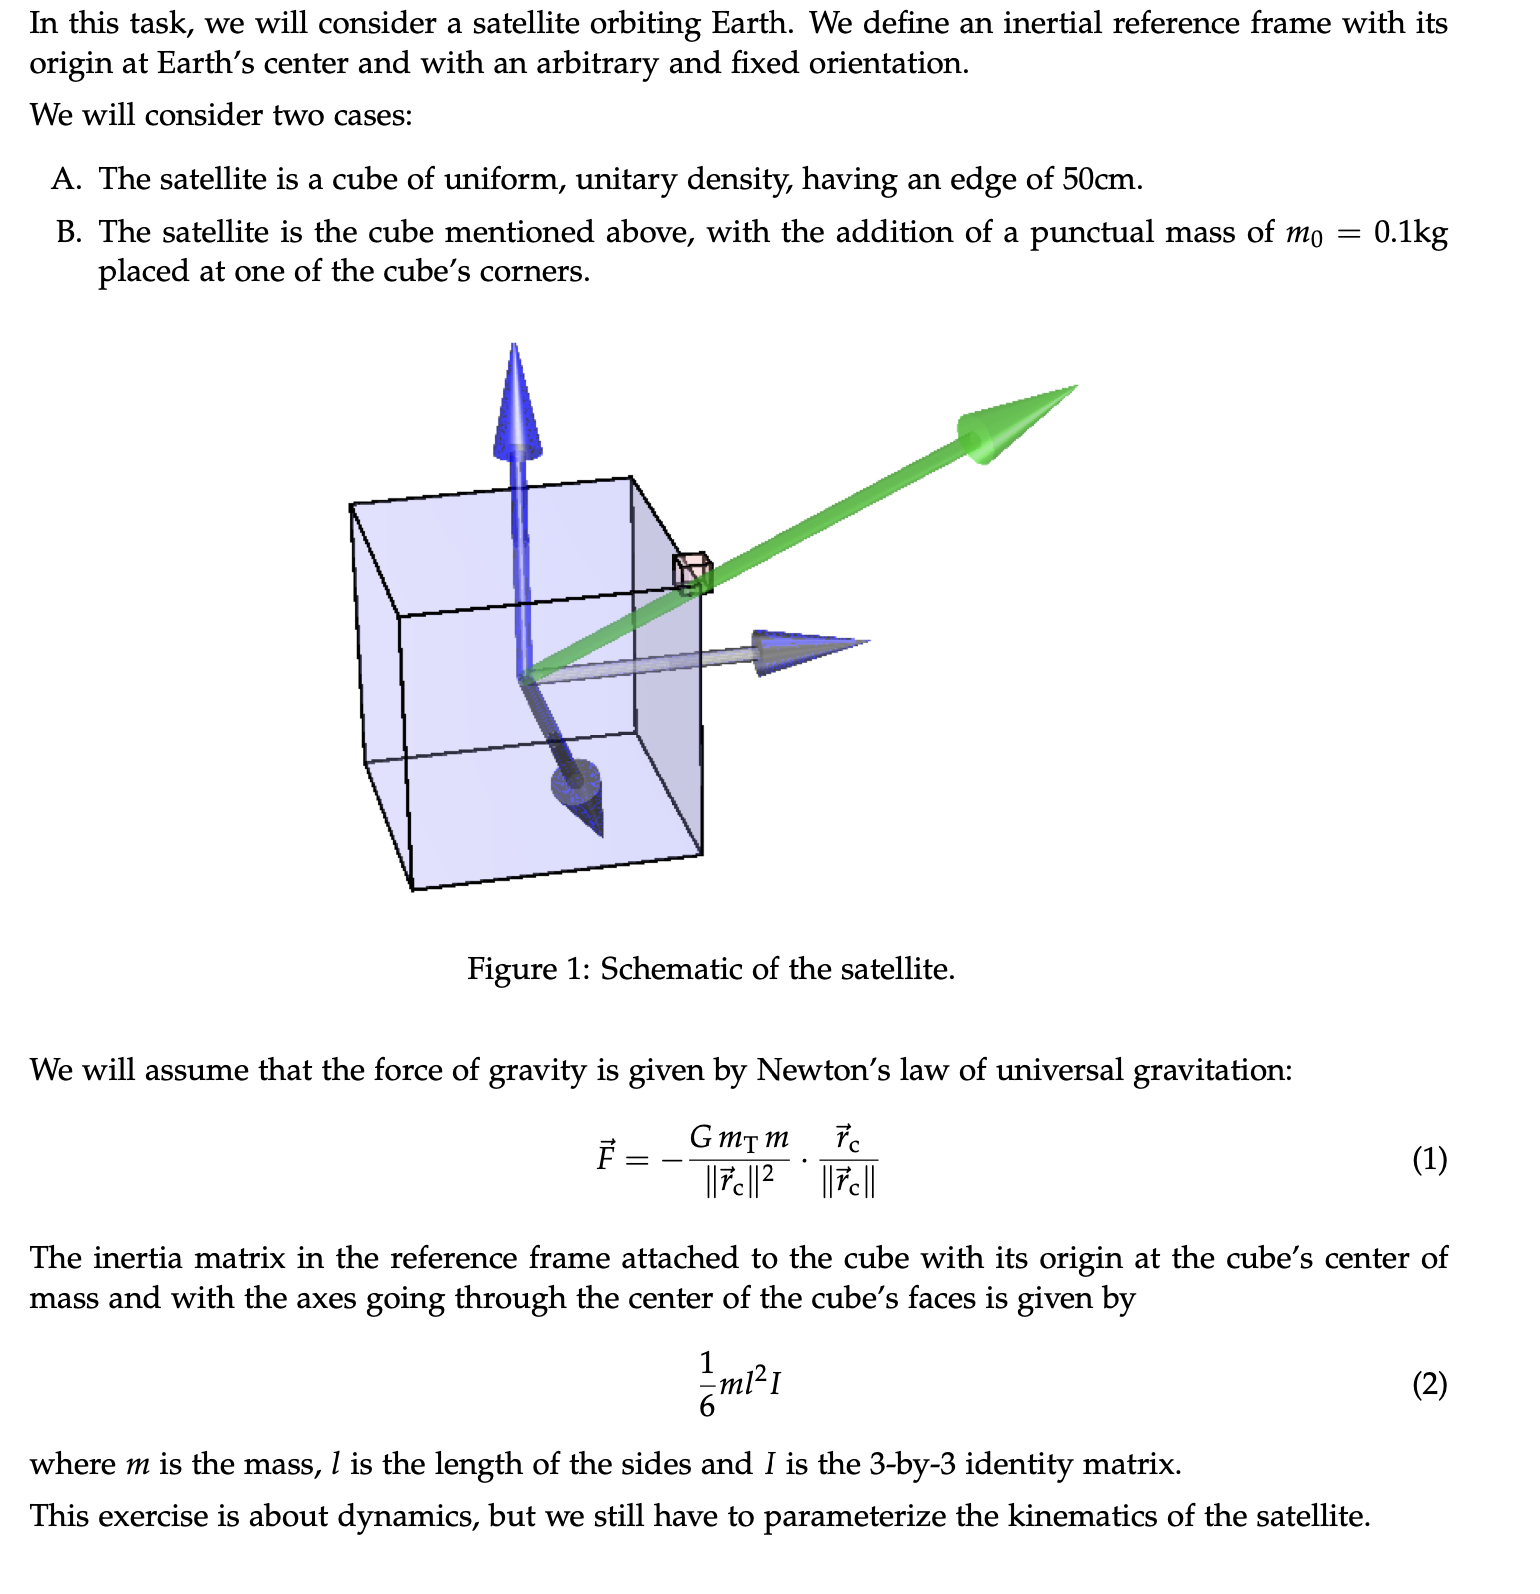
\includegraphics[scale = 0.5]{Skjermbilde 2024-05-23 kl. 18.56.18.png}
\end{figure}

(a) Consider the satellite without the added mass. Use the Newton-Euler equations to derive the dynamics of the satellite, i.e., find expressions for $\ddot{\mathbf{r}}_c^i$ and $\dot{\boldsymbol{\omega}}_{ib}^b$.
\\
\\

\textbf{Solution:} The Newton-Euler equations referenced to the center of mass are given by

\begin{equation}
    \mathbf{F}_{bc} = m \mathbf{a}_c
\end{equation}

\begin{equation}
    \mathbf{T}_{bc} = \mathbf{M}_{b/c} \cdot \boldsymbol{\alpha}_{ib} + \boldsymbol{\omega}_{ib} \times \left( \mathbf{M}_{b/c} \cdot \boldsymbol{\omega}_{ib} \right)
\end{equation}

\textcolor{gray}{Expressing the first equation in the inertial frame and the second in body frame gives}

\begin{equation}
    \ddot{\mathbf{r}}_c^i = \frac{\mathbf{F}^i}{m} = -\frac{G m T}{\|\mathbf{r}_c^i\|^2} \frac{\mathbf{r}_c^i}{\|\mathbf{r}_c^i\|}
\end{equation}

\begin{equation}
    \mathbf{M}_c^b \dot{\boldsymbol{\omega}}_{ib}^b = -\left( \boldsymbol{\omega}_{ib}^b \right)^\times \mathbf{M}_c^b \boldsymbol{\omega}_{ib}^b
\end{equation}

\textcolor{gray}{Note that we have used the fact that the gravitational force has zero moment around the center of mass.}
\\
\\
\textcolor{gray}{Further using that $\mathbf{M}_c^b = \frac{1}{6} m l^2 \mathbf{I}$ gives}

\begin{equation}
    \left( \boldsymbol{\omega}_{ib}^b \right)^\times \mathbf{M}_c^b \boldsymbol{\omega}_{ib}^b = \frac{1}{6} m l^2 \left( \boldsymbol{\omega}_{ib}^b \right)^\times \boldsymbol{\omega}_{ib}^b = 0
\end{equation}

\textcolor{gray}{Which gives the simplified expression}

\begin{equation}
    \ddot{\mathbf{r}}_c^i = -\frac{G m T}{\|\mathbf{r}_c^i\|^2} \frac{\mathbf{r}_c^i}{\|\mathbf{r}_c^i\|}
\end{equation}

\begin{equation}
    \dot{\boldsymbol{\omega}}_{ib}^b = 0
\end{equation}
\\
\\
\textbf{b)}
\\
\\
Now consider the added mass (case 2 above). The added mass will shift the center of mass of the system. Calculate the inertia matrix around this new center of mass and find the updated expressions for $\ddot{\mathbf{r}}_c^i$ and $\dot{\boldsymbol{\omega}}_{ib}^b$.
\\
\\
\textbf{Hint:} Use the parallel axis theorem to find the new inertia matrix.
\\
\\
\textbf{Solution:} To find the new inertia matrix with respect to the new center of mass, we first find the inertia matrix with respect to the old center of mass (the center of the cube) with the extra mass added. This is given by
\\
\\
\begin{equation}
    \mathbf{M}_0^b = \frac{1}{6} m l^2 \mathbf{I} - m_0 \left( \mathbf{r}_0^b \times \right) \left( \mathbf{r}_0^b \times \right),
\end{equation}
where $m_0$ is the added mass, and $\mathbf{r}_0$ is the vector from the center of the satellite to the added mass, i.e.,
\begin{equation}
    \mathbf{r}_0^b = \frac{l}{2}
    \begin{bmatrix}
        \pm 1 \\
        \pm 1 \\
        \pm 1
    \end{bmatrix} \quad \text{(the signs depend on the corner)}.
\end{equation}

In order to find the inertia matrix with respect to the center of mass, we have to first find the vector from the center of mass to the center of the cube, $\mathbf{r}_s$. We observe that the addition of a mass $m_0$ at a distance $L$ in one particular direction will shift the center of mass $\frac{m_0}{m + m_0} L$ units in that direction. Hence,
\begin{equation}
    \mathbf{r}_s^b = -\frac{m_0}{m_0 + m} \mathbf{r}_0^b,
\end{equation}
and the parallel axis theorem states
\begin{equation}
    \mathbf{M}_{b/o}^b = \mathbf{M}_{b/c}^b - (m + m_0) \left( \mathbf{r}_s^b \times \right) \left( \mathbf{r}_s^b \times \right) \implies \mathbf{M}_{b/c}^b = \mathbf{M}_{b/o}^b + (m + m_0) \left( \mathbf{r}_s^b \times \right) \left( \mathbf{r}_s^b \times \right).
\end{equation}
Which gives
\begin{equation}
    \mathbf{M}_c^b = \frac{1}{6} m l^2 \mathbf{I} - m_0 \left( \mathbf{r}_0^b \times \right) \left( \mathbf{r}_0^b \times \right) + (m + m_0) \left( \mathbf{r}_s^b \times \right) \left( \mathbf{r}_s^b \times \right).
\end{equation}

The dynamics are now given by
\begin{equation}
    \ddot{\mathbf{r}}_c^i = \frac{\mathbf{F}^i}{m + m_0} = -\frac{G m T}{\|\mathbf{r}_c^i\|^2} \frac{\mathbf{r}_c^i}{\|\mathbf{r}_c^i\|},
\end{equation}

\begin{equation}
    \mathbf{M}_c^b \dot{\boldsymbol{\omega}}_{ib}^b = -\left( \boldsymbol{\omega}_{ib}^b \right)^\times \mathbf{M}_c^b \boldsymbol{\omega}_{ib}^b.
\end{equation}

\textcolor{gray}{Note that we have used the fact that the gravitational force has zero moment around the center of mass. Further using that $\mathbf{M}_c^b = \frac{1}{6} m l^2 \mathbf{I}$ gives}
\begin{equation}
    \left( \boldsymbol{\omega}_{ib}^b \right)^\times \mathbf{M}_c^b \boldsymbol{\omega}_{ib}^b = \frac{1}{6} m l^2 \left( \boldsymbol{\omega}_{ib}^b \right)^\times \boldsymbol{\omega}_{ib}^b = 0,
\end{equation}

\subsection{Pseudo code for Implicit Runge-Kutta}
\begin{figure}[H]
    \centering
    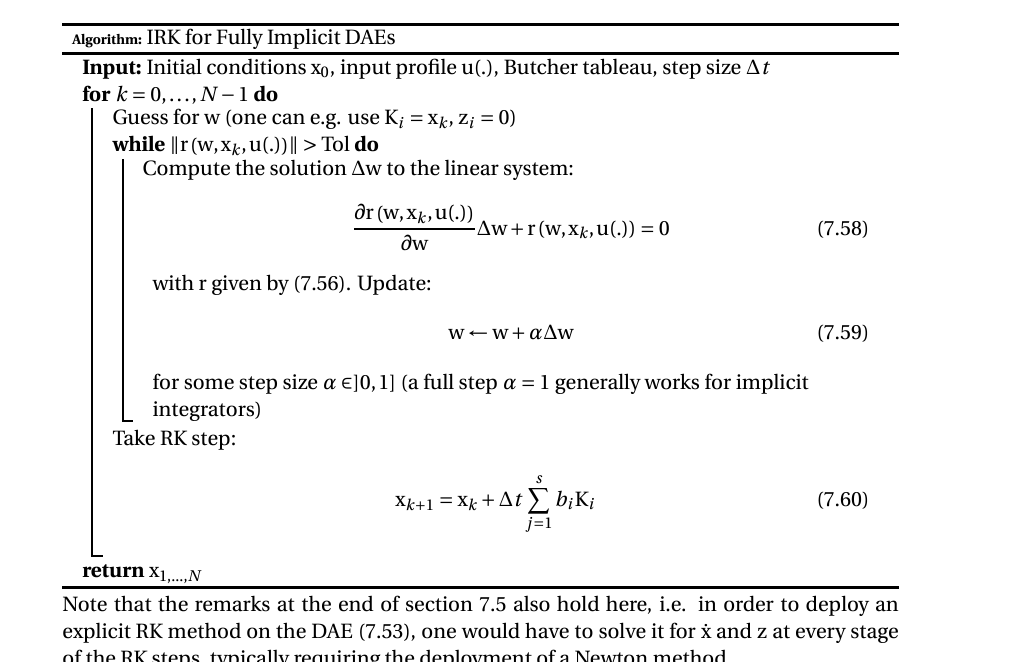
\includegraphics[scale = 0.5]{figures/IRK psedo code.png}
    \caption{IRK pseudo code, find more on page 144 in Gros}
\end{figure}

\subsection{Kinetic Energy of ball on beam}

\begin{figure}[H]
    \centering
    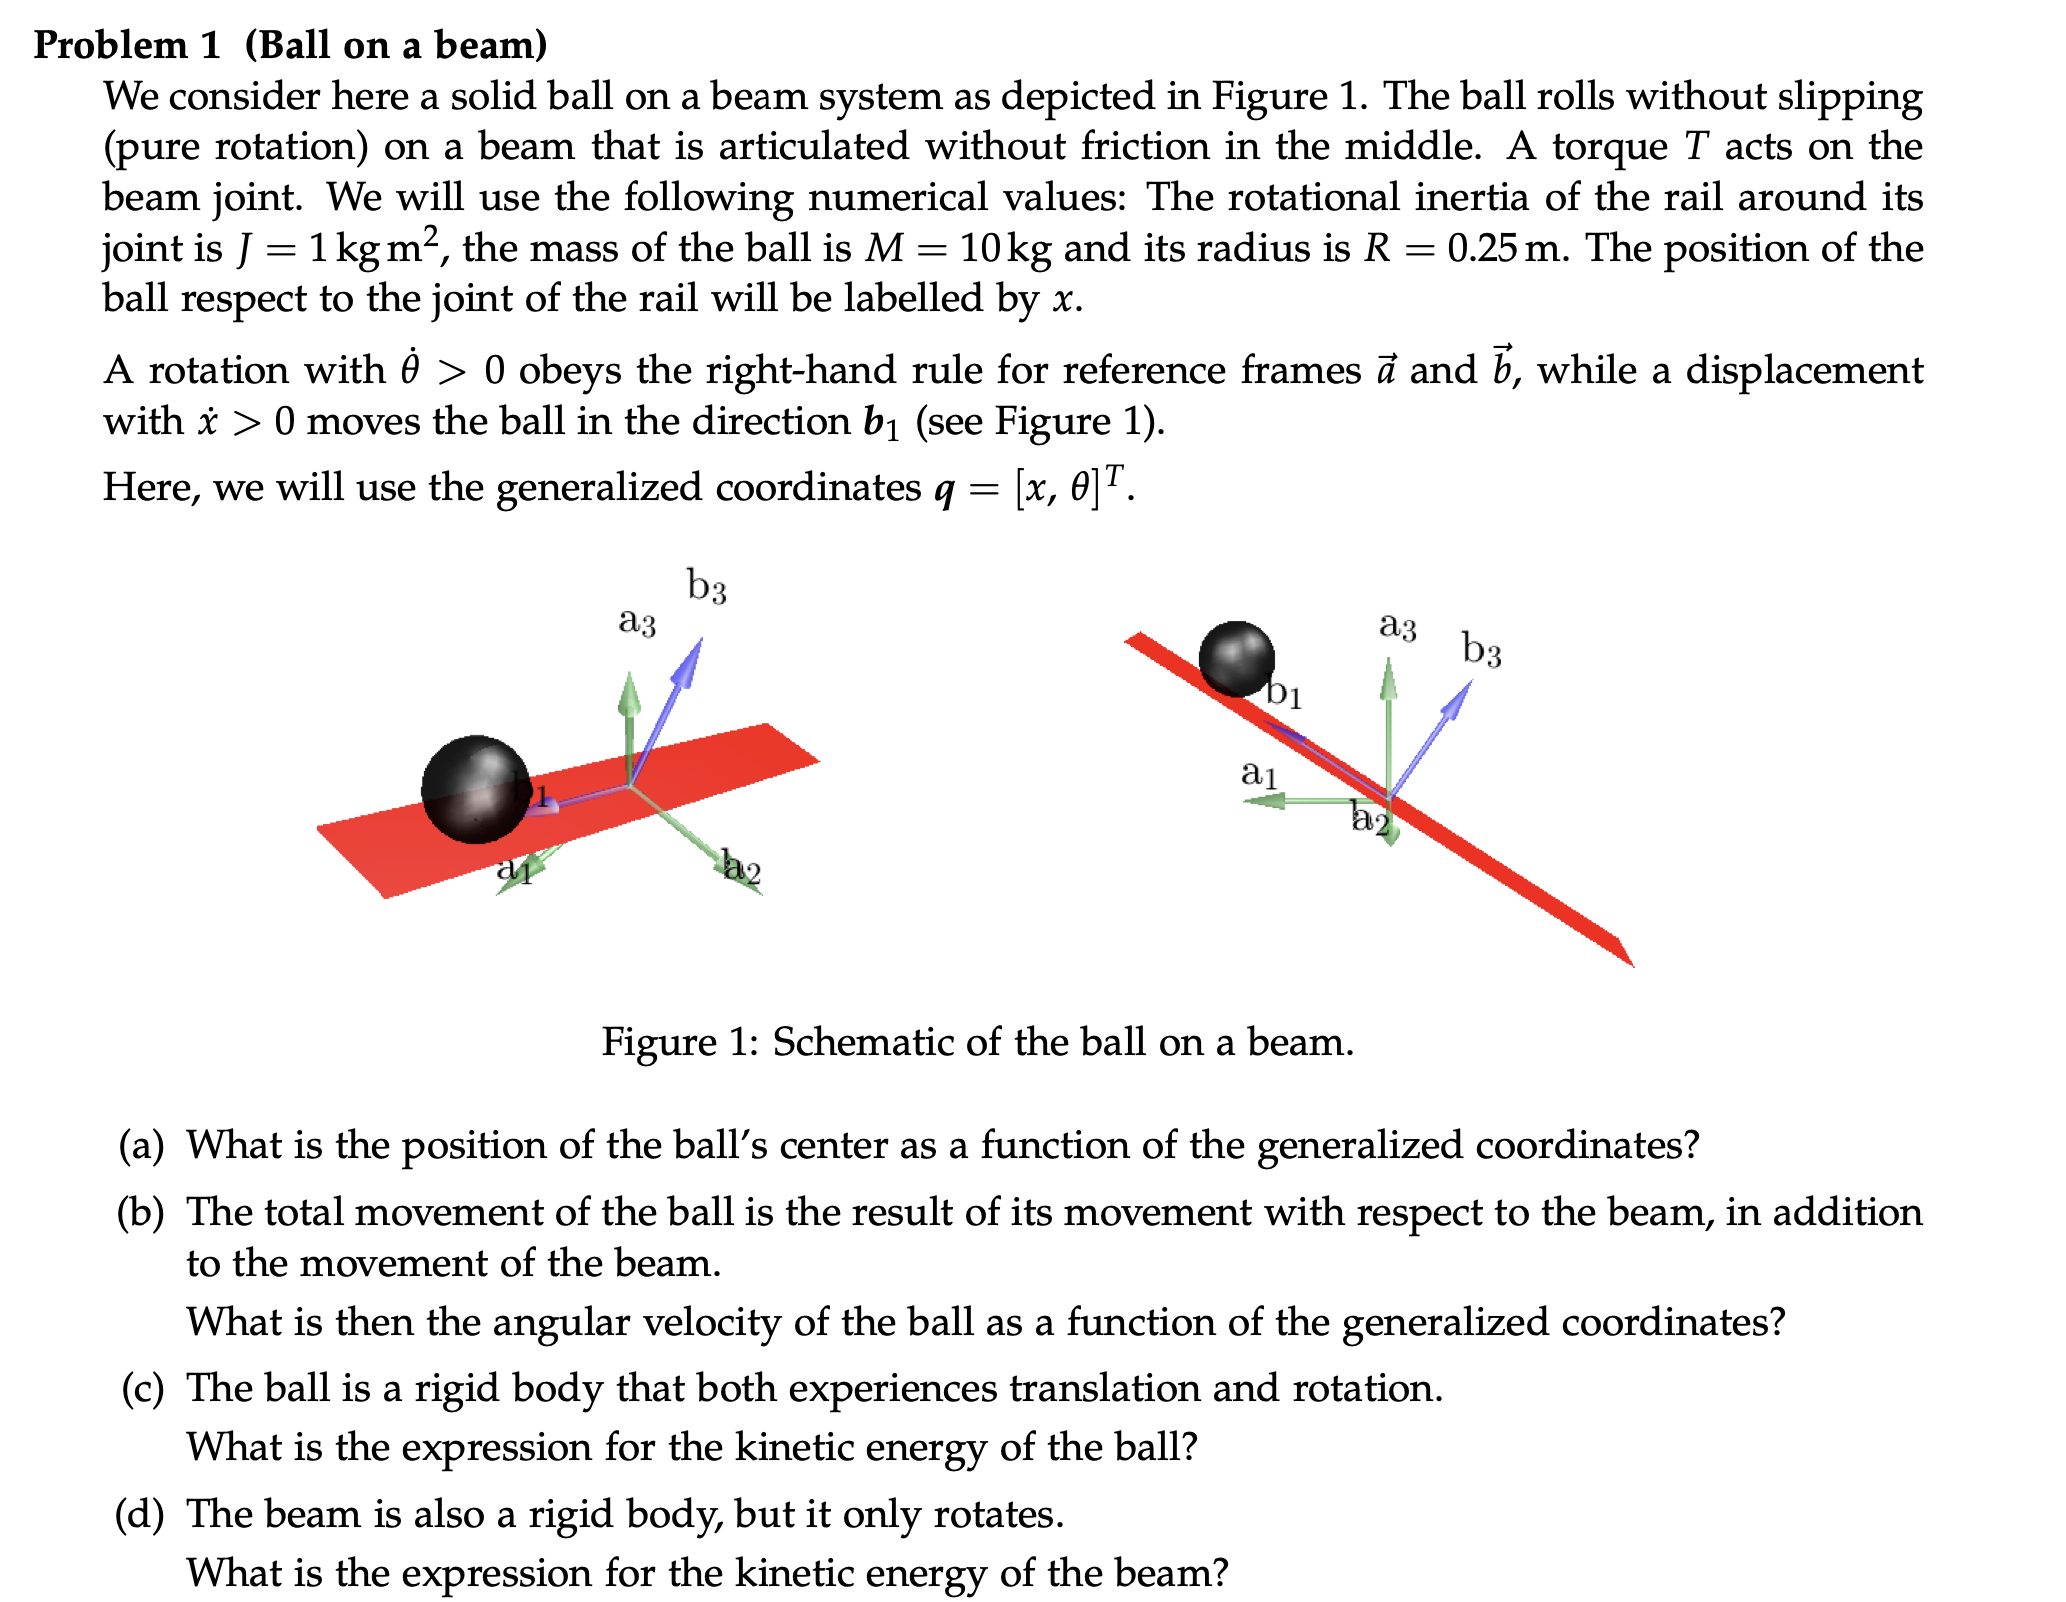
\includegraphics[scale = 0.4]{Skjermbilde 2024-05-24 kl. 10.57.23.png}
    \caption{Caption}
    \label{fig:enter-label}
\end{figure}

\textbf{(a) The position of the center of mass of the ball as a function of the generalized coordinates is given by:}
\begin{equation}
\mathbf{p} = x \begin{bmatrix} \cos \theta \\ \sin \theta \end{bmatrix} + R \begin{bmatrix} -\sin \theta \\ \cos \theta \end{bmatrix}
\end{equation}

\textbf{(b) The angular velocity of the ball as a function of the generalized coordinates is:}
\begin{equation}
\omega = \dot{\theta} + \frac{\dot{x}}{R}
\end{equation}

\textbf{(c) The kinetic energy of the ball, which experiences both translation and rotation, is given by:}

\textit{Translational Kinetic Energy}
\begin{equation}
T_T(q, \dot{q}) = \frac{1}{2} \dot{\mathbf{q}}^T M_T(q) \dot{\mathbf{q}}, \quad M_T(q) = M \frac{\partial \mathbf{p}}{\partial \mathbf{q}}^T \frac{\partial \mathbf{p}}{\partial \mathbf{q}}
\end{equation}

\textit{Rotational Kinetic Energy}
\begin{equation}
T_R(q, \dot{q}) = \frac{1}{2} I_{\text{ball}} \omega^2, \quad I_{\text{ball}} = \frac{2}{5} M R^2
\end{equation}

\textit{Total Kinetic Energy}
\begin{equation}
T(q, \dot{q}) = T_T + T_R
\end{equation}

\textbf{(d) The kinetic energy of the beam, which only rotates, is given by:}
\begin{equation}
T_r(q, \dot{q}) = \frac{1}{2} J \dot{\theta}^2
\end{equation}

\textbf{Overall Kinetic Energy}
\begin{equation}
T(q, \dot{q}) = T_T + T_R + T_r
\end{equation}

\textbf{Potential Energy}
\begin{equation}
V(q) = Mg p(2) = Mg (x \sin \theta + R \cos \theta)
\end{equation}

\textbf{Generalized Forces}
\begin{equation}
\mathbf{Q} = \begin{bmatrix} 0 \\ T \end{bmatrix}
\end{equation}


\subsection{Pendelum Lagrange example}

\begin{figure}[H]
    \centering
    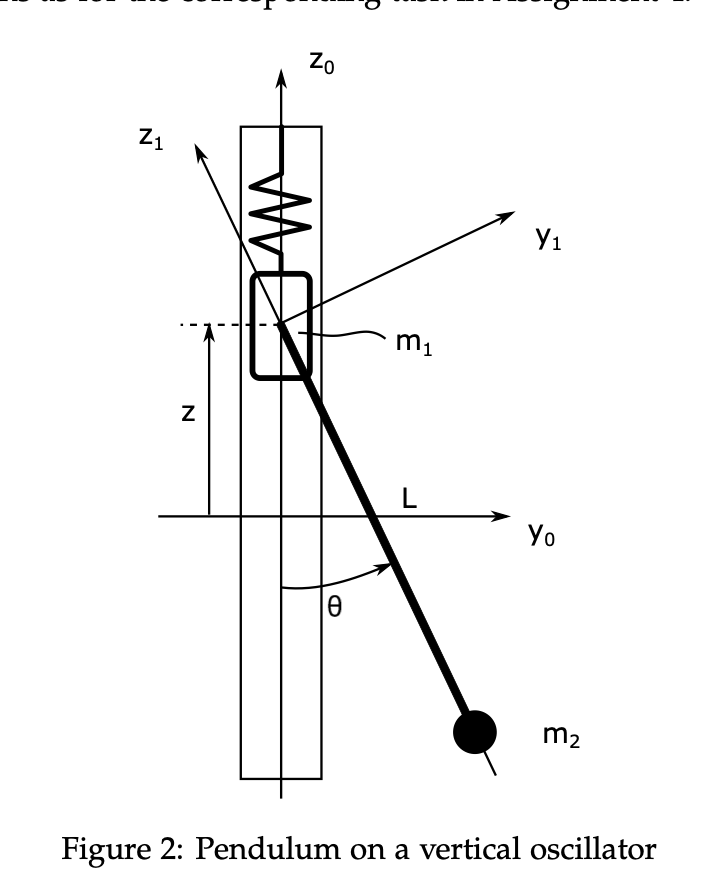
\includegraphics[scale = 0.4]{Skjermbilde 2024-05-24 kl. 14.32.36.png}
    \caption{Caption}
    \label{fig:enter-label}
\end{figure}

\textbf{a)} Select a set of generalized coordinates. 
\\
\\
solution: \[vec{q} = [z, \theta]^T\]
\\
\\
\textbf{b)} Find the kinetic energy of the system and express it in terms of the generalized coordinates (and their time derivatives).
\\
\\
\textbf{Solution:} To find the kinetic energy as a function of the generalized coordinates (and their time derivatives) we need to find the velocity components of the masses. We will express the coordinates of the masses in terms of the generalized coordinates and then differentiate. For \(m_1\), only the \(z\)-coordinate is relevant. As seen in the figure, the variable \(z\) is the \(z\)-coordinate of \(m_1\).
\\
\\
Mass \(m_2\) has the following coordinates:
\[
y_2 = L \sin \theta
\]
\[
z_2 = z - L \cos \theta
\]
\\
\\
Differentiating our 3 coordinates, gives
\[
\dot{z}_1 = \dot{z}
\]
\[
\dot{y}_2 = L \cos \theta \dot{\theta}
\]
\[
\dot{z}_2 = \dot{z} + L \sin \theta \dot{\theta}
\]
\\
\\
The kinetic energy can then be found as
\[
T = \frac{1}{2} m_1 \dot{z}_1^2 + \frac{1}{2} m_2 \dot{y}_2^2 + \frac{1}{2} m_2 \dot{z}_2^2
\]
\[
= \frac{1}{2} (m_1 + m_2) \dot{z}^2 + \frac{1}{2} L^2 m_2 \dot{\theta}^2 + L m_2 \dot{\theta} \dot{z} \sin \theta
\]
\\
\\
\textbf{c)} Find the potential energy of the system and express it in terms of the generalized coordinates.
\\
\\
\textbf{Solution:} The potential energy has three contributions. The first and second contribution is related to the energy storage from elevating the masses in the gravitational field, and the third contribution comes from compressing or stretching the spring. The following expression represents these contributions:
\\
\\
\[
V = z m_1 g + (z - L \cos \theta) m_2 g + \frac{1}{2} kz^2
\]
\\
\\
\textbf{d:} Find equations of motion for the system.
\\
\\
\textbf{Solution:} We start by finding the partial derivative of the kinetic energy with respect to each of the generalized rates:
\[
\frac{\partial T}{\partial \dot{z}} = (m_1 + m_2) \dot{z} + L m_2 \dot{\theta} \sin \theta
\]
\[
\frac{\partial T}{\partial \dot{\theta}} = L^2 m_2 \dot{\theta} + L m_2 \dot{z} \sin \theta
\]

We then find the time derivatives of the above expressions:
\[
\frac{d}{dt} \left( \frac{\partial T}{\partial \dot{z}} \right) = (m_1 + m_2) \ddot{z} + L m_2 \ddot{\theta} \sin \theta + L m_2 \dot{\theta}^2 \cos \theta
\]
\[
\frac{d}{dt} \left( \frac{\partial T}{\partial \dot{\theta}} \right) = L^2 m_2 \ddot{\theta} + L m_2 \ddot{z} \sin \theta + L m_2 \dot{z} \dot{\theta} \cos \theta
\]

We proceed by finding the partial derivatives of the kinetic energy with respect to the generalized coordinates:
\[
\frac{\partial T}{\partial z} = 0
\]
\[
\frac{\partial T}{\partial \theta} = L m_2 \dot{\theta} \dot{z} \cos \theta
\]

and the partial derivatives of the potential energy with respect to the generalized coordinates
\[
\frac{\partial V}{\partial z} = (m_1 + m_2) g + k z
\]
\[
\frac{\partial V}{\partial \theta} = L m_2 g \sin \theta
\]

Finally we use the Lagrange formula
\[
\frac{d}{dt} \left( \frac{\partial T}{\partial \dot{q}_i} \right) - \frac{\partial T}{\partial q_i} + \frac{\partial V}{\partial q_i} = 0
\]

Filling in the expressions found above gives
\[
\frac{d}{dt} \left( \frac{\partial T}{\partial \dot{z}} \right) - \left( \frac{\partial T}{\partial z} - \frac{\partial V}{\partial z} \right) = 0
\]
\[
\frac{d}{dt} \left( \frac{\partial T}{\partial \dot{\theta}} \right) - \left( \frac{\partial T}{\partial \theta} - \frac{\partial V}{\partial \theta} \right) = 0
\]
\[
L^2 m_2 \ddot{\theta} + L m_2 \ddot{z} \sin \theta + L m_2 \dot{z} \dot{\theta} \cos \theta + L m_2 g \sin \theta = 0
\]



\newpage
\subsection{Angular accelration}

\subsubsection{Klikka gyroscope}
Taks: find the angular accelration of the disk in 1-frame of this monstrocity.

\begin{figure}[H]
    \centering
    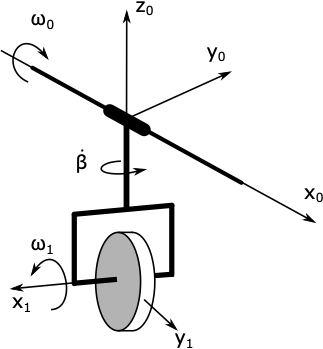
\includegraphics[scale = 0.7]{figures/klikka_eksempel.png}
    \caption{Klikka gyroscope}
    \label{fig:hardcoregyro}
\end{figure}

You can either use the formula for angular accelration or you can find the agular velocity of the disk in a completely stationary frame and then differentiate it. The 0-frame in the picture is not stationary so we introduce a new i-frame that is stationary. Because of $\omega_0$ the 0-frame is rotated $\theta_0$ in the negative direction of the $x_0/x_i$-axis from the i-frame.
The angular velocity of the disk expressed in diffrent frames are given by:
\begin{equation}
    -\omega_0\vec{i_i} + \dot{\beta}\vec{k_0} + \omega_1 \vec{i_1}
\end{equation}
transforming everything to the i-frame gives:
\begin{equation}
    \begin{bmatrix}
        -\omega_0 \\
        0\\
        0
    \end{bmatrix}
    +
    R_x(-\theta_0)
    \begin{bmatrix}
        0 \\
        0\\
        \dot{\beta}
    \end{bmatrix}
    +
    R_x(-\theta_0)R_z(\beta)
    \begin{bmatrix}
        \omega_1 \\
        0\\
        0
    \end{bmatrix}
\end{equation}

Now we can differentiate and transform back to the 1-frame:
\begin{equation}
    \alpha^1 =
    R_z(-\beta)
    R_x(\theta_0)
    \frac{d}{dt}
    \left(
    \begin{bmatrix}
        -\omega_0 \\
        0\\
        0
    \end{bmatrix}
    +
    R_x(-\theta_0)
    \begin{bmatrix}
        0 \\
        0\\
        \dot{\beta}
    \end{bmatrix}
    +
    R_x(-\theta_0)R_z(\beta)
    \begin{bmatrix}
        \omega_1 \\
        0\\
        0
    \end{bmatrix}
    \right)
\end{equation}
using that $\dot{\theta_0} = \omega_0$ we get:
\begin{equation}
    \alpha^1 =
    \begin{bmatrix}
        \omega_0\dot{\beta}\sin\beta\\
        \omega_1\dot{\beta}+ \omega_0\dot{\beta}\cos\beta\\
        \ddot{\beta}-\omega_0\omega_1\sin\beta
    \end{bmatrix}
\end{equation}
\newpage
\subsubsection{Klikka Gyroscope 2}
Taks: find the angular accelration of the disk in 1-frame of this monstrocity.

\begin{figure}[H]
    \centering
    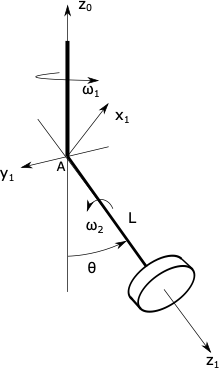
\includegraphics[scale = 0.7]{figures/gyro.png}
    \label{fig:hardcoregyro2}
\end{figure}

The fucked up thing here is that the angle between 1 and 0-frame is $\pi$ + $\theta$ and not $\theta$. Also the 1-frame is not stationary. We first define a completely stationary i-frame such that the 0-frame is rotated $\phi$ from the i-frame about the z-axis.
The angular velocity of the disc:
\begin{equation}
    \omega_1\vec{k_i} + \dot{\theta}\vec{j_1} + \omega_2 \vec{k_1}
\end{equation}
Then we express everything in the i-frame:
\begin{equation}
    \begin{bmatrix}
        0 \\
        0\\
        \omega_1
    \end{bmatrix}
    +
    R_z(\phi)
    \begin{bmatrix}
        0 \\
        \dot{\theta}\\
        0
    \end{bmatrix}
    +
    R_z(\phi)R_y(\theta+\pi)
    \begin{bmatrix}
        0 \\
        0\\
        \omega_2
    \end{bmatrix}
\end{equation}

Then we diffrentiate and rotate to 1-frame:
\begin{equation}
\alpha^1 =
    R_y(-\theta-\pi)
    R_z(-\phi)
    \frac{d}{dt}
    \left(
    \begin{bmatrix}
        0 \\
        0\\
        \omega_1
    \end{bmatrix}
    +
    R_z(\phi)
    \begin{bmatrix}
        0 \\
        \dot{\theta}\\
        0
    \end{bmatrix}
    +
    R_z(\phi)R_y(\theta+\pi)
    \begin{bmatrix}
        0 \\
        0\\
        \omega_2
    \end{bmatrix}
    \right)
\end{equation}
using that $\dot{\phi} = \omega_1$ we get:
\begin{equation}
    \alpha^1 =
    \begin{bmatrix}
        \omega_2\dot{\theta}+\omega_1\dot{\theta}\cos\theta \\
        \ddot{\theta} - \omega_1\omega_2\sin\theta \\
        \omega_1\dot{\theta}\sin{\theta}
    \end{bmatrix}
\end{equation}
\\
\\
\\

Did you find the muffin?



